%The default article class is limited to 12pt, but you can go up to 14, 17 or 20 points if you use the extarticle class:
\documentclass[a4paper,14pt]{extarticle}
\usepackage{cmap} %make LaTeX PDF output copy-and-pasteable
\usepackage[T2A]{fontenc}
\usepackage[utf8]{inputenc} %coding
\usepackage[english,ukrainian]{babel}
\usepackage{amssymb,amsfonts,amsmath,cite,enumerate,float}
\usepackage{indentfirst} %set an additional space before a paragraph at the begining of new section
\usepackage{graphicx}
\usepackage{wrapfig}
\usepackage{varwidth}
\usepackage{setspace}

\usepackage[table,xcdraw]{xcolor}

\usepackage{hyperref}
\definecolor{linkcolor}{HTML}{0000FF}
\definecolor{urlcolor}{HTML}{0000FF} 
\hypersetup{pdfstartview=FitH, linkcolor=linkcolor, urlcolor=urlcolor, colorlinks=true}

\graphicspath{{Screenshots/}} %path to images

\parskip=1mm %space between paragraphs

\usepackage{geometry} 
\geometry{left=1.25cm}
\geometry{right=1.25cm}
\geometry{top=1cm}
\geometry{bottom=2cm}

\begin{document}

\begin{titlepage}
    \newpage

    \begin{minipage}[c]{\linewidth}

        \newlength{\maxpreambula}
        \settowidth{\maxpreambula}{\small{<<Київський політехнічний інститут імені Ігоря Сікорського>>}}    

        \hspace{5cm}\parbox{\maxpreambula}{
            \begin{spacing}{1.1}\small{
                Міністерство освіти і науки України \\
                Національний технічний університет України \\
                <<Київський політехнічний інститут імені Ігоря Сікорського>> \\
                Навчально-науковий фізико-технічний інститут }
            \end{spacing}
        }
            
        \vspace*{-2.35cm}
        \hspace*{1.5cm}
        
\includegraphics[width=0.13\paperwidth]{kpi_emblem.png}

    \end{minipage}
    
    \vspace{\fill}
    
    \begin{center}
        \begin{spacing}{1.5}
            \textbf{\Large{Реалізація EM-алгоритму}} \\ 
            \vspace{1cm}\textbf{\normalsize{предмет <<Марковські моделі та їхнє застосування>>}}
        \end{spacing}
    \end{center}
    
    \vspace{\fill}
    
    \newlength{\maxname}
    \settowidth{\maxname}{\small{Цибульник Антон Владиславович}}

    \hfill\parbox{\maxname}{
        \begin{spacing}{1.1}
            \small{\textbf{Роботу виконав:}} \\ 
            \small{Студент групи ФІ-91,} \\
            \small{Цибульник Антон Владиславович} \\
        \end{spacing}
    }

    \hfill\parbox{\maxname}{
        \begin{spacing}{1.1}
            \small{\textbf{Роботу перевірила:}} \\ 
            \small{Ніщенко Ірина Іванівна} \\
        \end{spacing}
    }

    \vspace{0.5cm}

    \begin{center}
        \small{2022}
    \end{center}
    
\end{titlepage}

%\tableofcontents

\newpage

%\addcontentsline{toc}{section}{Мета}
\section*{Мета}
Отримати базові навички по використанню AWS Management Console та
створити власний мікро-сервер для подальшого використання.

%\addcontentsline{toc}{section}{Завдання}
\section*{Завдання} 

\begin{itemize}
    \item Реєстрація в AWS;
    \item Створення власного віртуального мікро-сервера;
    \item Отримання віддаленого доступу через SSH;
    \item Вивчення елементів моніторингу серверу та налаштування;
    \item Документування зробленої роботи у вигляді деталізованого протоколу з коментарями.
\end{itemize}

%\addcontentsline{toc}{section}{Хід виконання роботи}
\section*{Хід виконання роботи}

%\addcontentsline{toc}{subsection}{Реєстрація в AWS}
\subsection*{1. Реєстрація в AWS}

Для реєстрації в AWS слід перейти за 
\href{https://portal.aws.amazon.com/billing/signup#/start}{посиланням}.
На сторніці реєстрації спершу необхідно послідовно заповнити поля 
пошти та імені акаунту (Рис. \ref{fig:start}), надалі пройти ще 4 кроки 
реєстрації, один з яких буде присвячений реквізитам банківської карти.

\begin{figure}[H]
    \center{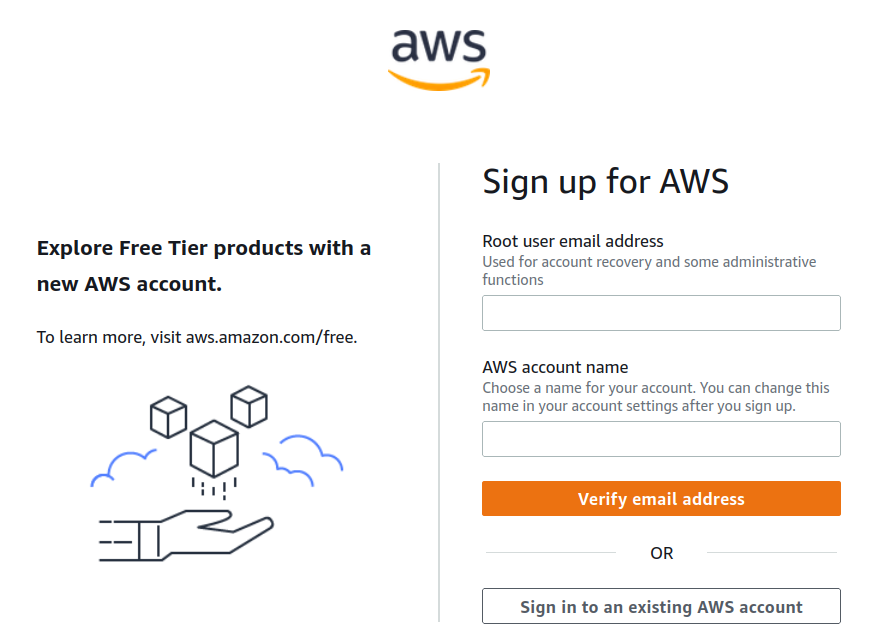
\includegraphics[width=0.75\linewidth]{1.png}}
    \caption{Перший етап реєстрації}
    \label{fig:start}
\end{figure}

\subsection*{2. Створення мікро-інстансу}

\begin{wrapfigure}[8]{r}{0.45\linewidth}
    \vspace{-1.7cm}
    \center{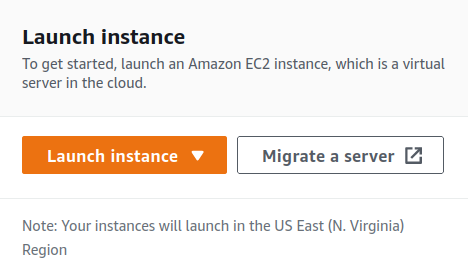
\includegraphics[width=0.9\linewidth]{2.png}}
    \caption{Запуск мікро-інстансу}
    \label{fig:instance}
\end{wrapfigure}

Після реєстрації в AWS стає доступним пакет Amazon Management Console 
із цілим спектром сервісів. Обираємо сервіс Elastic Computing 
Service (EC2). З EC2 маємо можливість запустити новий віртуальний 
сервер, тобто інстанс. Для цього слід натиснути помаранчеву кнопку 
Launch Instance, як зображено на Рис.~\ref{fig:instance}. \\

Далі для остаточного створення інстансу необхідно пройти такі кроки\footnote
{\href{https://drive.google.com/file/d/1bw8HWLhrWmIfW7_4GhIvwFP40NiJpqZz/view}
{детально у 3 розділі книги <<Amazon Web Services in Action>> 
авторів Andreas Wittig, Michael Wittig.}}:

\begin{enumerate}
    \item \textbf{Choose an Amazon Machine Image (AMI):} 
    the first step is to choose a bundle of an OS and 
    preinstalled software for your virtual server, 
    called an Amazon Machine Image (AMI). I selected 
    Ubuntu Server 20.04 LTS (HVM).
    \item \textbf{Choose an instance type:} I selected t2micro (Free tier Only).
    \item \textbf{Configure instance details:} I selected all the options by default.
    \item \textbf{Add storage:} I selected all the options by default.
    \item \textbf{Tag instance:} Tags help you to organize resources on AWS. A tag
    is nothing more than a key-value pair. I added a <<Name>> tag to 
    my resources to help me find my stuff later. I used <<Name>> as 
    the key and <<myserver>> as the value.
    \item \textbf{Configure security group:} I selected all the options by default.
    \item \textbf{Review the instance launch} for the virtual server.
\end{enumerate}

\subsection*{3. Отримання доступу до нього}

Після завершення створення інстансу слід створити пару 
ключів RSA. Наприклад, я створив ключ з ім'ям <<lab>> 
та зберіг наданий файл {\ttfamily lab.pem} на жорсткому 
диску свого комп'ютера. Після успішного створення інстанс 
з’явиться серед списку активних (як на Рис. \ref{fig:active instance}).

\begin{figure}[h]
    \center{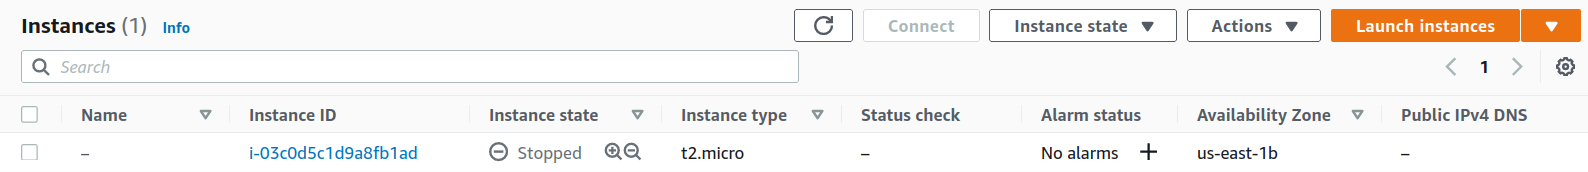
\includegraphics[width=1\linewidth]{3.1.png}}
    \caption{Перелік активних інстансів}
    \label{fig:active instance}
\end{figure}

Доступ до інстансу можно отримати прямо з браузера, 
через через ssm manager або SSH client. Для операційної 
системи мого комп'ютера (Ubuntu 20.04) я обрав спосіб 
доступу до сервера через SSH client. У результаті введення 
необхідних команд у термінал (інструкції на Рис. 
\ref{fig:connect to instance}), я отримав бажаний доступ 
до сервера (Рис. \ref{fig:connect to instance by termanal}).

\begin{figure}[h]
    \center{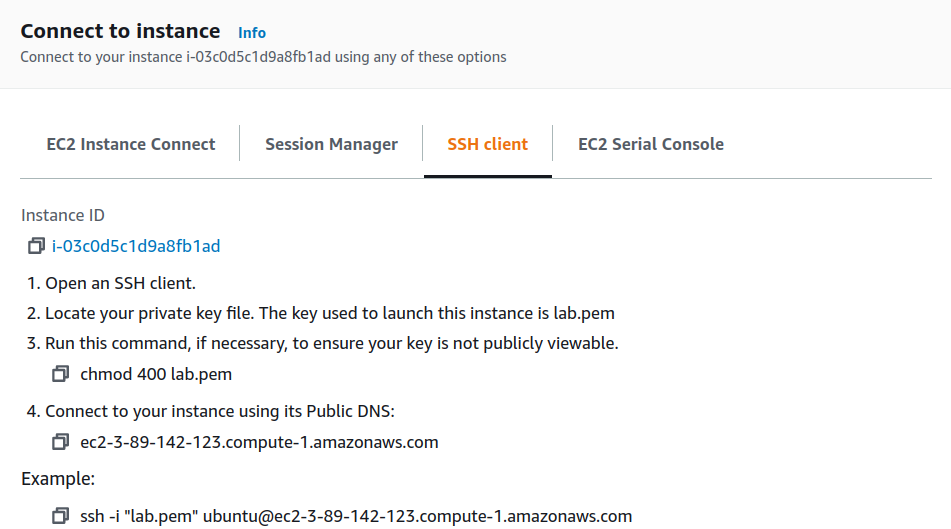
\includegraphics[width=1\linewidth]{3.2.png}}
    \caption{Інструкції приєднання через SSH client}
    \label{fig:connect to instance}
\end{figure}

\begin{figure}[H]
    \center{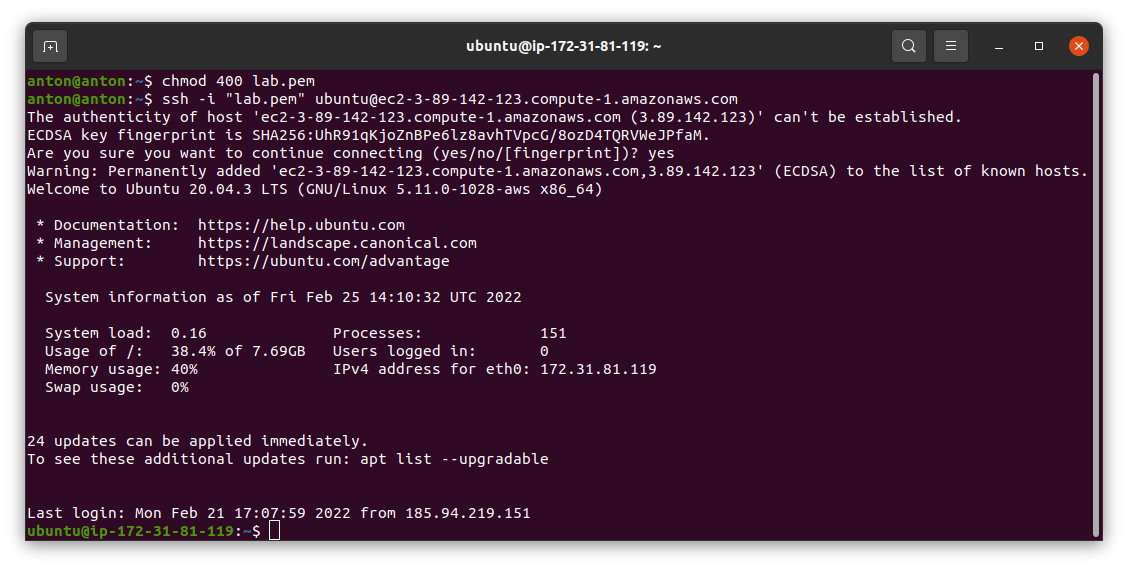
\includegraphics[width=1\linewidth]{3.3.png}}
    \caption{Отримання доступу через термінал}
    \label{fig:connect to instance by termanal}
\end{figure}

\subsection*{4. Моніторинг використання ресурсів}

Нажче наведено перелік команд, за допомогою яких було 
здійснено моніторинг використання ресурсів на інстансі.

\begin{figure}[h]
    \center{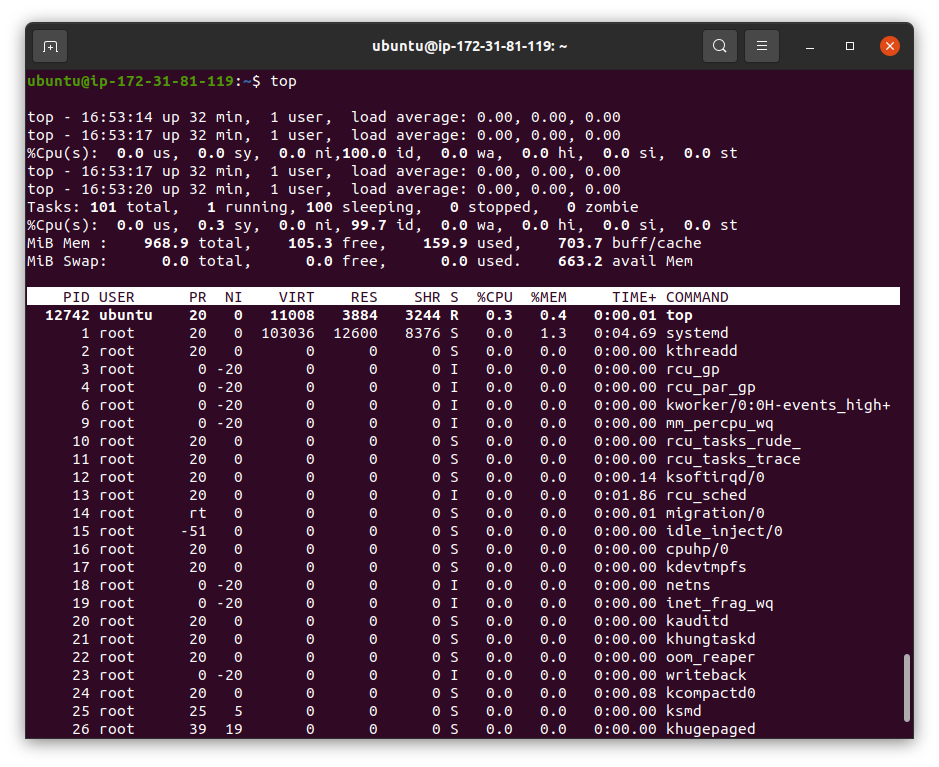
\includegraphics[width=1\linewidth]{4.1.png}}
    \caption{Моніторинг ресурсів командою top}
    \label{fig:top}
\end{figure}

\begin{figure}[H]
    \center{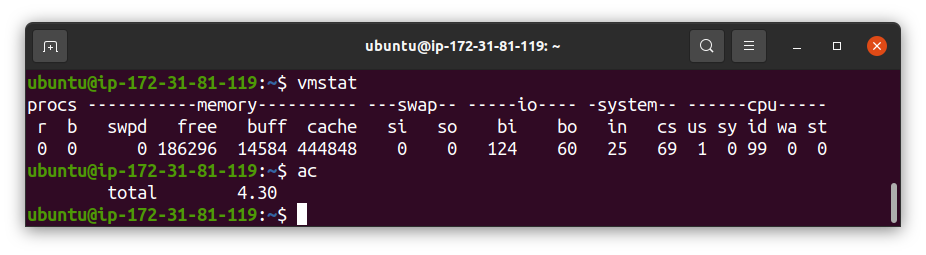
\includegraphics[width=1\linewidth]{4.2.png}}
    \caption{Моніторинг ресурсів командами vmstat та ac}
    \label{fig:vmstat & ac}
\end{figure}

\begin{figure}[H]
    \center{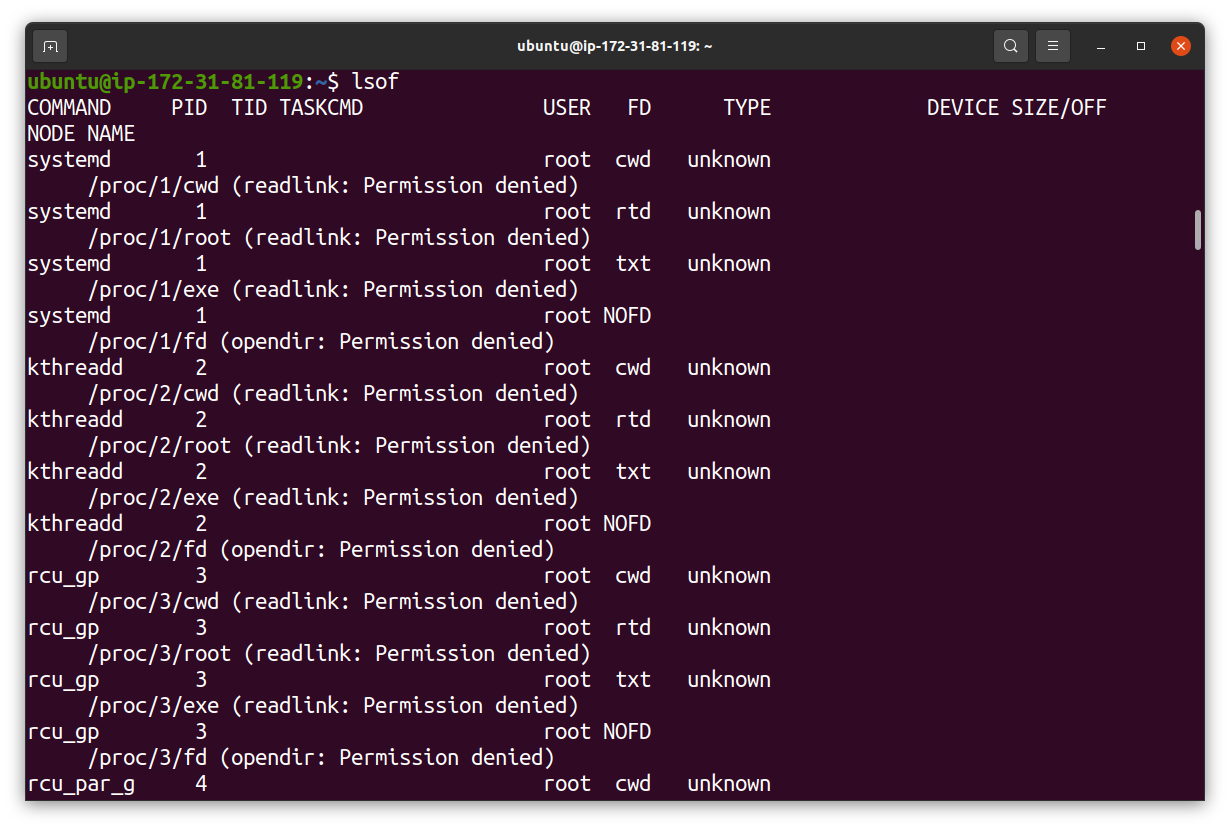
\includegraphics[width=1\linewidth]{4.3.png}}
    \caption{Моніторинг ресурсів командою lsof}
    \label{fig:lsof}
\end{figure}

\begin{figure}[H]
    \center{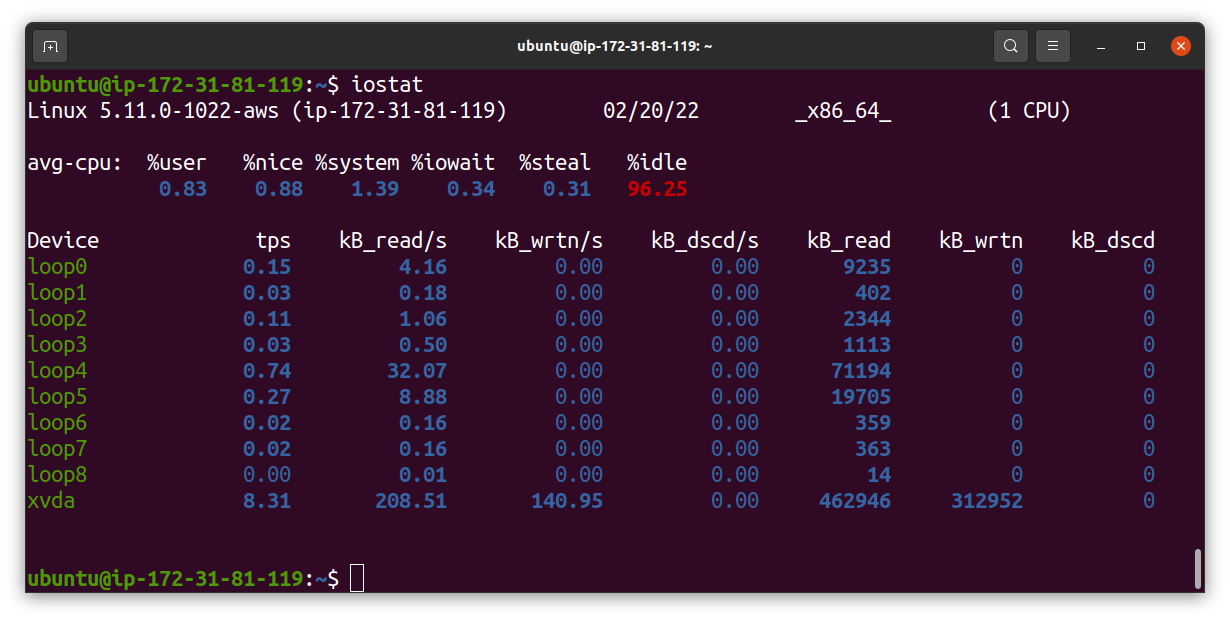
\includegraphics[width=1\linewidth]{4.4.png}}
    \caption{Моніторинг ресурсів командою iostat}
    \label{fig:iostat}
\end{figure}

\begin{figure}[H]
    \center{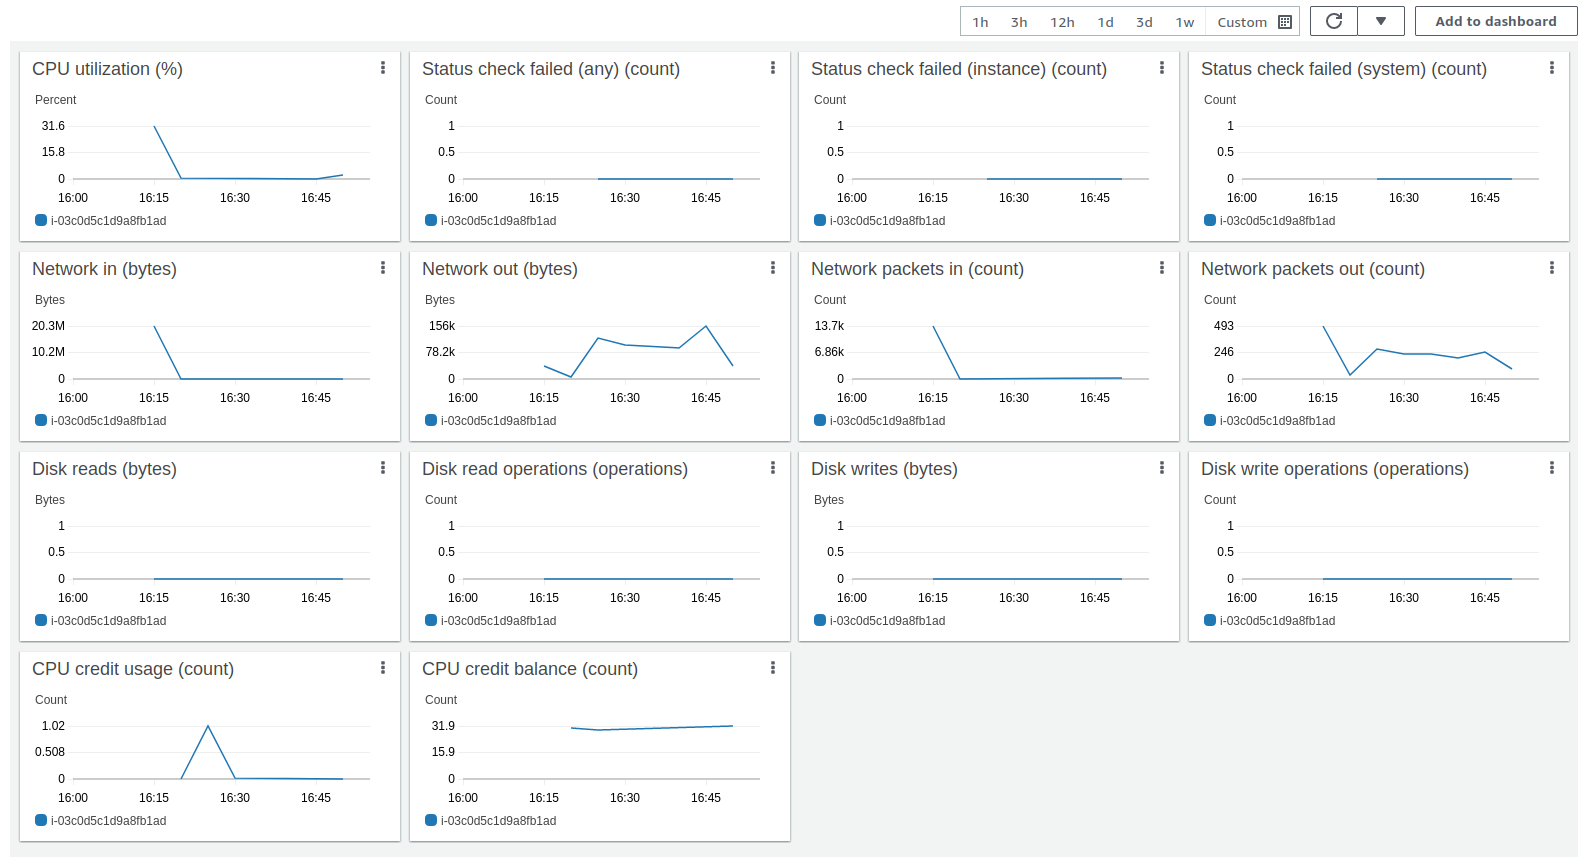
\includegraphics[width=1\linewidth]{4.6.png}}
    \caption{Моніторинг ресурсів безпосередньо через сайт AWS}
    \label{fig:monitoring}
\end{figure}

\subsection*{5. Завантаження файлу на інстанс}
\label{section:5}

Наступним завданням було завантажити файли на інстанс, а саме:
створити на локальному сховищі пустий файл {\ttfamily *.txt} й завантажити 
його на інстанс через термінал та за допомогою програмного забеспечення FileZilla.

\subsubsection*{Завантаження через FileZilla}

За допомогою команди {\ttfamily sudo apt install -y filezilla} на операційну 
систему Ubuntu 20.04 було завантажено програмне забеспечення FileZilla. 
Запустивши програму, слід було виконати такі кроки налаштування:

\begin{enumerate}
    \item Обрати на панелі інструментів Edit $\rightarrow$ Settings $\rightarrow$ SFTP;
    \item Натиснути Add key file $\rightarrow$ обрати відповідний файл-ключ $\rightarrow$ OK;
    \item Обрати на панелі інструментів File $\rightarrow$ Site Manager $\rightarrow$ New site;
    \item На панелі праворуч ввести Host (ваш Public DNS), Port (22), Protocol (SFTP) та значення User (ubuntu);
    \item Натиснути Connect.
\end{enumerate}

Після цього з'являться всі необхідні інструменти для завантаження файлу з локального 
сховища на інстанс. Для цього необхідно лише <<перетягнути>> файли з лівої панелі 
на праву (Рис. \ref{fig:move by FileZilla}).

\begin{figure}[h]
    \center{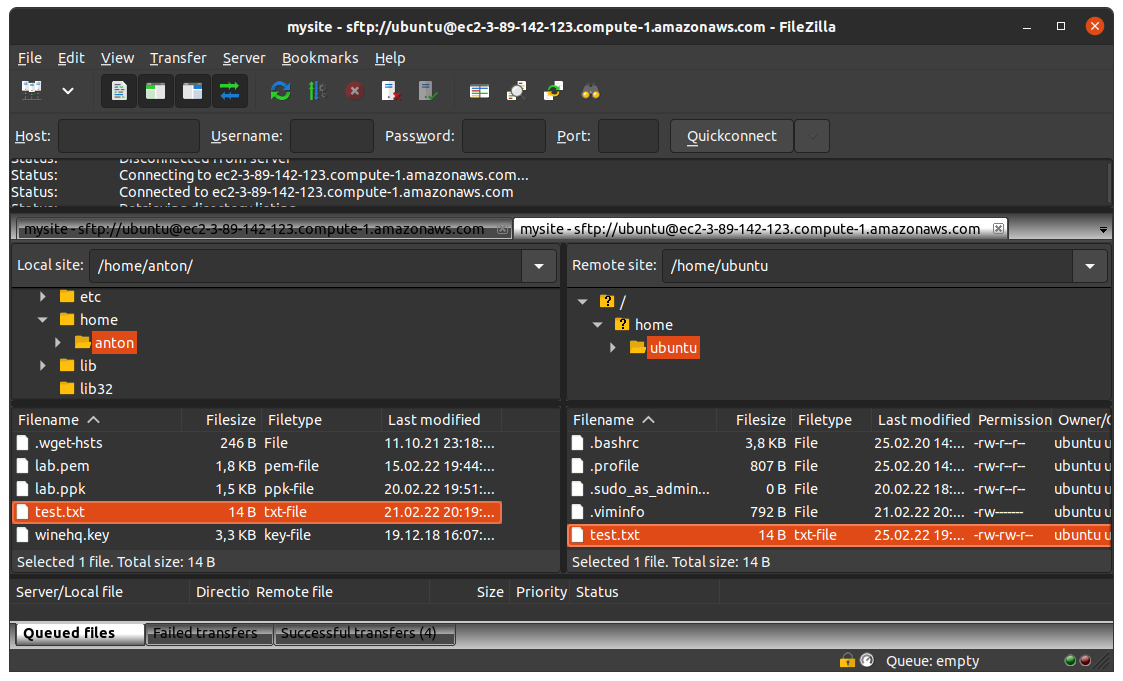
\includegraphics[width=1\linewidth]{5.5.png}}
    \caption{Завантаження через FileZilla}
    \label{fig:move by FileZilla}
\end{figure}

\subsubsection*{Завантаження через термінал}

Перш за все виникла потреба встановити на локальне сховище 
пакет інструментів {\ttfamily putty}. Для цього була використана команда 
{\ttfamily sudo apt install -y putty}. Далі за допомогою утиліти {\ttfamily pscp} 
було завантажено створений раніше файл {\ttfamily test.txt} на інстанс. 
Проте варто зазначити, що для справної роботи цієї утиліти файл-ключ {\ttfamily lab.pem} 
слід було перетворити у розширенні {\ttfamily lab.ppk}. Остаточно, командою 
{\ttfamily ls} було перевірено успішне виконання завдання. Результати наведено на 
Рис. \ref{fig:move by terminal}.

\begin{figure}[H]
    \begin{minipage}[H]{1\linewidth}
        \center{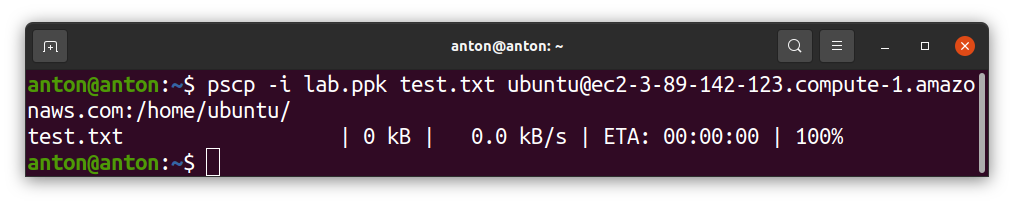
\includegraphics[width=1\linewidth]{5.7.1.png}}
    \end{minipage}
    \vfill
    \begin{minipage}[H]{1\linewidth}
        \center{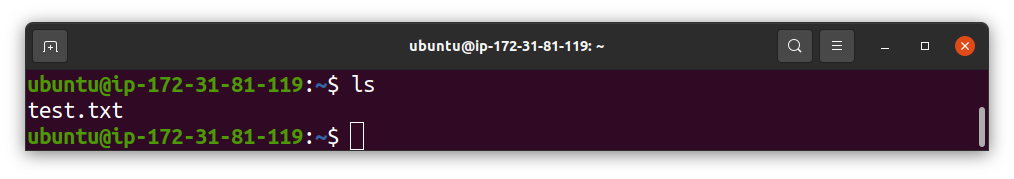
\includegraphics[width=1\linewidth]{5.7.2.png}}
        \caption{Завантаження через термінал}
        \label{fig:move by terminal}
    \end{minipage}
\end{figure}

\subsection*{6. Відкриття файлу на інстансі}

Тепер можемо перейти до відкриття файлу на інстансі за допомогою 
редактора Vim. Крім того, за допомогою цього редактора необхідно 
додати текст <<Hello world!>> у раніше перенесений на сервер файл. 

Перейшовши за 
\href{https://www.geeksforgeeks.org/getting-started-with-vim-editor-in-linux/}{посиланням}, 
можна довідатися більше про можливості Vim. Проте, наразі цікавлять
лише команди відкриття та редагування файлів. Послідовність дій 
для виконання поставленого завдання:

\begin{enumerate}
    \item На інстансі відкрити файл в редакторі Vim за допомогою введення 
    комнади {\ttfamily vim test.txt} у терміналі;
    \item Для редагування файлу ввести через клавіатуру символ {\ttfamily i};
    \item Написати текст {\ttfamily <<Hello, world!>>};
    \item Щоб вийти з режиму редагування, натиснути клавішу Esc;
    \item Зберегти написане введенням з клавіатури через двокрапку команди {\ttfamily :wq!}.
\end{enumerate}

Для перевірки успішного виконання можна знову відкрити файл через команду 
{\ttfamily vim test.txt} й переконатися, що він не порожній. Альтернативою
буде використання команди {\ttfamily cat test.txt} для перегляду вмісту файлу 
прямо через термінальне вікно (як на Рис. \ref{fig:vim}). Детальніше про команду 
{\ttfamily cat} за 
\href{https://askubuntu.com/questions/642942/what-is-cat-used-for}{посиланням}.

\begin{figure}[H]
    \begin{minipage}[H]{1\linewidth}
        \center{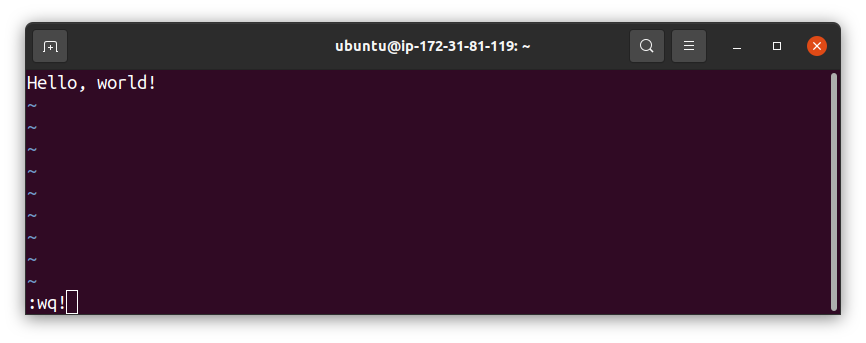
\includegraphics[width=1\linewidth]{6.1.png}}
    \end{minipage}
    \vfill
    \begin{minipage}[H]{1\linewidth}
        \center{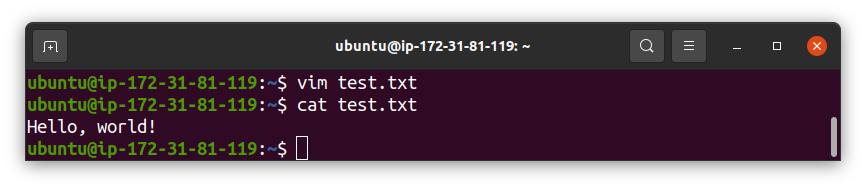
\includegraphics[width=1\linewidth]{6.2.png}}
        \caption{Робота з редактором Vim}
        \label{fig:vim}
    \end{minipage}
\end{figure}

\subsection*{7. Завантаження зміненого файлу}

Останнім кроком завантажимо змінений файл з інстансу на локальне сховище.
Зробити це можна двома способами, які вже було розглянуто на 
сторінці \pageref{section:5}. Я скористаюся способом завантаження 
через термінал, як це показано на Рис. \ref{fig:upload}.

\begin{figure}[H]
    \center{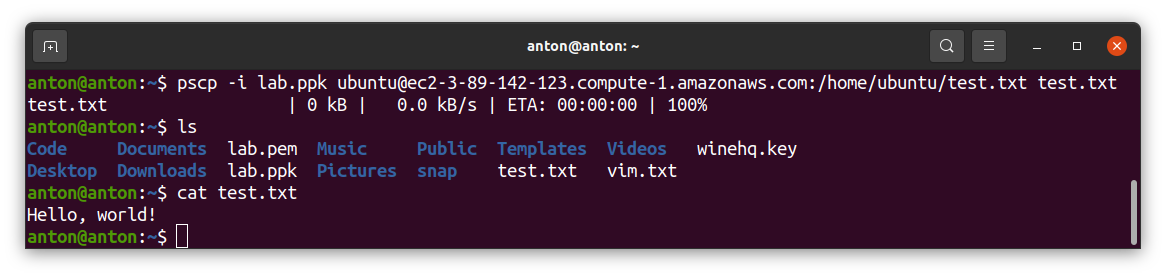
\includegraphics[width=1\linewidth]{7.png}}
    \caption{Завантаження файлу з інстансу на локальне сховище}
    \label{fig:upload}
\end{figure}

\subsection*{8. Перелік проблем протягом виконання роботи}

\begin{enumerate}
    \item Під час реєстрації акаунту в AWS я зіткнувся з проблемою на 
    підґрунті введення даних про банківську карту. На жаль, карту було 
    заблоковано, цитую: \\
     
    \parbox{\linewidth}{\textit{<<Нещодавно за Вашою карткою було зафіксовано 
    підозрілі операції, що могли виявитися шахрайськими. На жаль, ми не змогли 
    зв’язатися з Вами за номерами телефонів, які Ви залишали в банку, 
    щоб прояснити ситуацію. Тому з метою безпеки Вашу картку було тимчасово 
    заблоковано>>}} \\

    Звернувшись у відділення банку, мою карту розблокували. 

    \item Для моніторингу використання ресурсів за допомогою команди {\ttfamily ac}
    додатковим кроком встановив цю утиліту: {\ttfamily sudo apt install acct}.

    \item Під час спроб знайти способи завантаження файлу на інстанс 
    довелося перетворювати файл-ключ у розширення {\ttfamily *.ppk}. 
    За допомогою команди {\ttfamily sudo puttygen pemKey.pem -o ppkKey.ppk -O private} 
    не вдалося коректро перетворити файл, термінал Ubuntu відмовлявся сприймати оновлене розширення. 
    Був вимушений просити допомоги у користувачів операційної системи Win\-dows. 
    Додатково вказавши при перетворенні необхідну версію, таки вдалося отримати бажаний результат. 

    \item Як уже зазначалося раніше, у тому ж розділі завантаження файлу на інстанс для 
    використання утиліти {\ttfamily pscp} мусив додатково завантажувати пакет інструментів 
    {\ttfamily putty} такою командою: {\ttfamily sudo apt install -y putty}.
\end{enumerate}

\end{document}